\section{Crowds}
\label{sec:crowds}
In this section, we establish some concepts for discussing the behaviour of 
crowds in general, in order to have a basis on which we can analyse our chosen 
model. We also give an overview of the work that has been done in the field of 
crowd modelling and which approaches there has been to tackling this area, as 
well as background information on the type of model (agent-based) we are 
dealing with. Finally, we outline the cases we want to use in our simulations.

\subsection{Agent-based models and their origin}
The modelling of human behaviour using agent-based models is a 
pretty new field in modelling \cite{helbing00}. In this section, we give an 
overview of the use of agent-based models in other areas.

An agent-based model is a model that describes the behaviour of individuals 
and through simulations derive behaviour of the system being modelled.  
Agent-based models are used in many different fields.  They have their origin 
in physics where the idea of agent-based models dates as far back as 1820. 
Back then Laplace wrote \cite{simintro}:

% TODO: Language cleanup etc.

\begin{quote}
    An intelligent being who, at a given moment, knows all the forces that 
    cause nature to move and the positions of the objects that it is made 
    from, if also it is powerful enough to analyze this data, would have 
    described in the same formula the movements of the largest bodies of the 
    universe and those of the lightest atoms. Although scientific research 
    steadily approaches the abilities of this intelligent being, complete 
    prediction will always remain infinitely far away.
\end{quote}

So the main idea of agent-based models and their application has been thought 
of since long before the usage of computers. But it wasn't until the last half 
of the 20th century that it was actually possible to work with agent models 
because of the numbers of calculations needed to make use of 
them \cite{simintro}.  Since then the application of agent-based models have 
been huge and it is now used in many of different fields. 

One of the most well-known and first established (1957 \cite{MDintro}) 
agent-based model simulations is the molecular dynamics (MD)-simulations 
\cite{MDintro}. The idea of MD-models is simply to describe particles moving 
around by calculating the mechanical forces working on each of the particles.  
These kind of models allow you too see what happens with each particle and from 
that it is possible to calculate well known physical properties like 
temperature, pressure and so on . You can even see when there is a phase 
change from liquid to solid and back again. But also you can use it for much 
more complex behavior. In molecular biology and chemistry you can use 
MD-simulations to calculate the behavior of long-chain molecules \cite{MDbio}.  
In these models you even sometime add some stochastic elements to the models.  
This can be used to get some theoretical idea about how reactions happens and 
alot of other things.

But also in fields that you normally wouldn't connect with physics you see the 
application of microscopic models.
One of the more exotic fields to use microscopic models is in financial 
markets \cite{finans}.  In these kind of simulations you can describe how the 
behavior of individuals affects market dynamics.  It is of course not 
mechanical forces that controls this kind of models, but the idea of looking 
at and calculate the effects of the individual is maintained. 

Microscopic models has also been used on different types of animals like fish 
and with good results.  One of the things that have been simulated is fish 
schools \cite{fish}. In these simulations they try to the describe how a fish 
school moves around by calculating the positions of each fish and the effects 
from its nearest neighbours. In these kind of models people get some realistic  
looking behaviours that looks like what you would see in nature. Because of 
this very wide application of agent based models it seems natural to assume 
that it also could be fitted to use on human behaviour. Especially since it can 
be used on other animals, even though it could be argued that you of course 
would expect animals behavior to be more primitive than that of humans and 
therefore more easy to model.  Since microscopic models is used in a lot of 
different ways they also looks very different. That is because only the main 
idea of looking at the individual repeats throughout all of the models. So even 
though microscopic models is used very widely there is still a lot to of 
calculations and considerations that changes when the field changes and 
therefore it is still non-trivial.

\subsection{Social Force models}
%	There should be an introduction to this section.. were going to compare the 		%
%	differnt ways of simulating crowds.. but wait then it's not only relevant for 		%
%	social force models. This might fit better into the Crowds section if its rewitten	%
%	correctly.																			%

%	Some history about the social force model might serve well as an introduction here	%
In this section we will first give a short presentation on Social Force models and their history,
and then compare the features of Social Force models with the features of other models that describes
the behavior of crowds.
\\

The idea behind social force models is that each individual, pedestrian $\alpha$, in the crowd acts 
on her own from a personal aim or goal and by behavioral reactions to the environment. 
Different forces such as other pedestrians, walls and obstacles are taken into account 
when pedestrian $\alpha$ walks toward her aim or goal, so that she does not walk 
into another pedestrian or wall. The forces influencing $\alpha$'s motion 
of direction are not forces acting on $\alpha$'s body, but has to be seen as a quantity 
that describes the motivation to act. Since $\alpha$ is used to the situations 
she is normally confronted with, her reactions will be rather automatic and 
determined by her experience of which reaction will be that best. Since the reaction 
is rather automatic it is possible to put the rules of pedestrian behavior into an equation 
of motion.\cite{social-force}

\subsection{Comparison with other crowd models}
There are other ways to model crowds than social force models such as Rule Based models, 
Cellular Automata models and Hybrid models. Below we will make a short explanation of each of the 
other crowd models, and then compare the features of the models.\\												%

\textbf{Rule Based models}\\
Rule Based models describe the movement of pedestrians through sets of basic rules. Each 
pedestrian apply collision detection and avoidance to prevent collision with other pedestrians. 
However they do not in general apply collision response, and therefore collisions and overlappping 
of the pedestrians may occur under some circumstances. Some models have applied stopping 
rules to prevent these situations.\cite{Comparison}

\textbf{Cellular Autamata models}\\
These models are discrete, deterministic and is made up of cells like the squares in a chessboard.
An artificial intelligence approach is used in Celluar Automata (CA) defined as mathematical idealisation 
of physical systems in which time and space are discrete, and physical quantities take a finite set of 
discrete values. Pedestrian can not collide since the floor is dicretised and the pedestrians can
only move to free adjecent cells.\cite{Comparison}

\textbf{Hybrid models}\\
The Hybrid models has been made from social force models and rule based models. 
The motion of the pedestrians is carried out like the social force models, but is also based 
on the psychological and geometrical rules. It preforms collision detection and response and rules 
are applied depending on the pedestrian's personality and the state of the environment. 
\cite{Comparison}
\\

\subsubsection{Geometrical features of the models}
Each of the different models have some geomatrical features relatively important and 
unimportant according to our simulation.

\textbf{Shaking} Wether pedestrians appear to shake when simulating the model. When 
simulating the social force models the pedestrians seems to shake when clogging and 
queues arise. This is caused by the modification of each pedestrians position in each 
time step. The Hybrid, CA and Rule Based model do not appear to shake while the simulation run.

\textbf{Discrete and Continuous movement} Wether the space and time are discretized. 
In the CA model the pedestrians move between discretized adjacent cells in one time step, 
and therefore have limited direction to go. The other models do not discretize space and 
therefore allow the pedestrians to move within continuous space.
 
\textbf{Overlapping} Wether overlapping of the pedestrians is possible. The rule 
based models and the CA models do have collision detection but not all have collision 
responce. The CA models have rules so that a pedestrian can not walk into an occupied 
cell, but if two pedestrians want to pass each other they step into the cell diagonal 
to their own cell, and in their way cross the other pedestrian in the intersection 
between the four cells. Newer models of the rule based and CA have made a stopping 
rule so that overlapping can not occur. The Hybrid and social force models do collision 
response to minimize the risk of overlapping. \cite{Comparison}

\begin{figure}
    \centering
    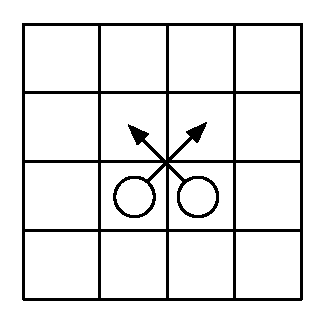
\includegraphics[scale=0.55]{Figures/Overlapping.pdf} 
    \caption[Overlapping]{Illustration of two agents overlapping in a CA model. The two agents can only walk to adjecent cells, and in
	     this case the agents crosses each other in their path to their next postition.}
    \label{Overlapping}
\end{figure}

\textbf{Pushing} Wether pedestrians can have physical contact. If the pedestrians 
can have physical contact they will be able to push each other in some direction. 
This ability is possible when using the Hybrid and the social force model. When 
simulating evacuations and chaotic events it has been observed that people do have 
physical contact and push each other \cite{self-org}.

\textbf{Communication} Wether the pedestrians can share information about the 
environment. The HiDAC and som newer rule based models allows the pedestrians 
to share information about the environment and to give orders. This feature is 
not included in social force models and CA. \cite{Comparison}

To illustrate different features of the different models the table below sums 
up the above mentioned.

\begin{center}
\begin{tabular}{lllll}
 & Social Forces & Rule Based & CA & Hybrid\\
Shaking avoidance     & - & + & + & +\\
Continuous space      & + & + & - & +\\
Overlapping avoidance & + & * & - & +\\
Pushing               & + & - & - & +\\
Communication         & - & * & - & +
\end{tabular}
\end{center}

Here + indicates that the feature is possible, - indicates it is not, and * that 
the model has been adjusted such that the feature have become possible. \cite{Comparison}

The features we are interested in and find relevant in our simulation are 
continuous space, pushing and overlapping avoidance. The continuous space is 
relevant for our simulaion to be as realistic as possible since we do not want 
our pedestrians to have at most nine directions to go each time step.
The feature of pushing is also important to include since in panic situation it 
has been seen that people push each. This feature will then make our simulation 
more realistic. The overlapping avoidance we find relevant since this enables 
pedestrians to walk through each other.

Therefore we find that modelling a crowd by using a social force model is most 
appropriate in our project. 
%	Finishing off with a conclusion would be neat					%


\subsection{Concepts for describing crowd behaviour}
In order to analyse the behavior of crowds, we need to establish some 
concepts to describe this behavior. It is not obvious which concepts  are 
useful when we need to distinguish between the results we get from our 
simulations. In this section we describe which concepts we use to describe the 
behavior of crowds, and why we have chosen them. This is based on the 
literature of crowd modeling.

One of the reasons for modeling crowds is to discover ways to make crowd 
situations safer for pedestrians, e.g. when evacuating a building in event of 
a fire. One of the main factors in this scenario is the \emph{efficiency} of 
the crowd movement. This is especially important when clearing a room in the 
event of a fire or other disaster: the faster everyone gets out, the lower is 
the chance of someone dying from flames or smoke.

Therefore it is important to know how the environment affects the efficiency 
of the crowd when it leaves the room. However we should specify how we intend 
measures the efficiency of a crowd.

The obvious measure of efficiency is measuring how long it takes to empty a 
given room. This, however, makes the results highly dependent on the specific 
situation we are modelling (i.e. room size, number of people in the room, 
etc.). Since it takes longer to empty a room of 10 people than it takes to
empty the very same room with 5 people. If we wish to compare results from 
different cases, we need a measure that is less dependent on the precise setup
of the simulation. Such a measure could be the average speed of a pedestrian 
compared to the desired one \cite{self-org}. Together with the \emph{flow rate}, 
i.e. the number of pedestrians passing a specific point (or line) in space per 
time unit. Further more we measure the density of the pedestrians in a certain 
area. These measures will tell us something about the efficiency of the crowd.

% TODO: This section needs to be expanded with more concepts, references to 
% where we get the concepts, as well as a better arguments for why we have 
% chosen exactly these measures.

\subsection{Our case(s)}
%introduction
In this section we outline which cases we want to simulate and why.
One of the main reasons for doing simulations is that we want to try to get 
a full understanding of the model. Doing simulations is a way to achieve this
understanding. Secondly we want to find any limitations and weaknesses of the 
model.

For this purpose we have thought about different scenarios that should make such 
limitations and weaknesses clear. We start by making a series of simple simulations
 where we can test isolated parts of the model and slowly increase the complexity 
of the simulations.

Basically there are three levels of the model we want to simulate. First we want to 
model a square room with an exit in the middle of one of the walls. In this 
room there will be a modest amount of people and no obstacles. The purpose of this 
simulation is to catch any early mistakes or misunderstandings in our implementation 
of the model.

From this we move on to varying the parameters of the model too see how the changes in 
in the these affect the behavior of the crowd in simple situations. This will
be done in the same simple simulation in order for us to have a transparent look 
at precisely what is going on. The results of these simulations will be compared 
with the value of the parameters presented in the literature.

After this we will test how the model handles different geometries of the environment. 
That is we will try to vary the shape of the room to see if the model starts producing 
unnatural crowd behavior as the complexity of the environment increases. 

In the end we will try so simulate more complicated situations to see if we can observe 
a range of self-organization phenomena that have been reported in the literature. 
These include clogging in bottlenecks, lane formation in bidirectional pedestrian 
flow and a faster-is-slower phenomena where some pedestrians end up moving slower than 
average because they are to impatient \cite{self-org}. Furthermore we want to test some phenomena 
that according to the literature should make the model break down. An example of this 
could be to model a situation of a room filled with smoke.   

All this should give a thorough idea about how this model should be handled and what parts 
of it that could be improved. or were you should be careful when using the model.

